\documentclass[]{article}
\usepackage{lmodern}
\usepackage{array}
\usepackage{float}
\usepackage{wrapfig}
\usepackage{graphicx}
\usepackage{booktabs}
\usepackage{amssymb,amsmath}
\usepackage{subfig}
\usepackage{caption}
\usepackage{ifxetex,ifluatex}
\usepackage{fixltx2e} % provides \textsubscript
\ifnum 0\ifxetex 1\fi\ifluatex 1\fi=0 % if pdftex
  \usepackage[T1]{fontenc}
  \usepackage[utf8]{inputenc}
\else % if luatex or xelatex
  \ifxetex
    \usepackage{mathspec}
  \else
    \usepackage{fontspec}
  \fi
  \defaultfontfeatures{Ligatures=TeX,Scale=MatchLowercase}
\fi
% use upquote if available, for straight quotes in verbatim environments
\IfFileExists{upquote.sty}{\usepackage{upquote}}{}
% use microtype if available
\IfFileExists{microtype.sty}{%
\usepackage{microtype}
\UseMicrotypeSet[protrusion]{basicmath} % disable protrusion for tt fonts
}{}
\usepackage[margin=1in]{geometry}
\usepackage{hyperref}
\hypersetup{unicode=true,
            pdftitle={Problem2},
            pdfborder={0 0 0},
            breaklinks=true}
\urlstyle{same}  % don't use monospace font for urls
\usepackage{graphicx,grffile}
\makeatletter
\def\maxwidth{\ifdim\Gin@nat@width>\linewidth\linewidth\else\Gin@nat@width\fi}
\def\maxheight{\ifdim\Gin@nat@height>\textheight\textheight\else\Gin@nat@height\fi}
\makeatother
% Scale images if necessary, so that they will not overflow the page
% margins by default, and it is still possible to overwrite the defaults
% using explicit options in \includegraphics[width, height, ...]{}
\setkeys{Gin}{width=\maxwidth,height=\maxheight,keepaspectratio}
\IfFileExists{parskip.sty}{%
\usepackage{parskip}
}{% else
\setlength{\parindent}{0pt}
\setlength{\parskip}{6pt plus 2pt minus 1pt}
}
\setlength{\emergencystretch}{3em}  % prevent overfull lines
\providecommand{\tightlist}{%
  \setlength{\itemsep}{0pt}\setlength{\parskip}{0pt}}
\setcounter{secnumdepth}{0}
% Redefines (sub)paragraphs to behave more like sections
\ifx\paragraph\undefined\else
\let\oldparagraph\paragraph
\renewcommand{\paragraph}[1]{\oldparagraph{#1}\mbox{}}
\fi
\ifx\subparagraph\undefined\else
\let\oldsubparagraph\subparagraph
\renewcommand{\subparagraph}[1]{\oldsubparagraph{#1}\mbox{}}
\fi

%%% Use protect on footnotes to avoid problems with footnotes in titles
\let\rmarkdownfootnote\footnote%
\def\footnote{\protect\rmarkdownfootnote}

%%% Change title format to be more compact
\usepackage{titling}

% Create subtitle command for use in maketitle
\newcommand{\subtitle}[1]{
  \posttitle{
    \begin{center}\large#1\end{center}
    }
}

\setlength{\droptitle}{-2em}

  \title{Problem2}
    \pretitle{\vspace{\droptitle}\centering\huge}
  \posttitle{\par}
    \author{}
    \preauthor{}\postauthor{}
    \date{}
    \predate{}\postdate{}
  
\usepackage{wrapfig}

\begin{document}
\maketitle

\subsection{(a)Explore the demographic information of the
customers.}\label{aexplore-the-demographic-information-of-the-customers.}

  After analysis, we regard \textbf{Age, Experience, Income, Family} and \textbf{Education} as demographic variables. Below are our results.

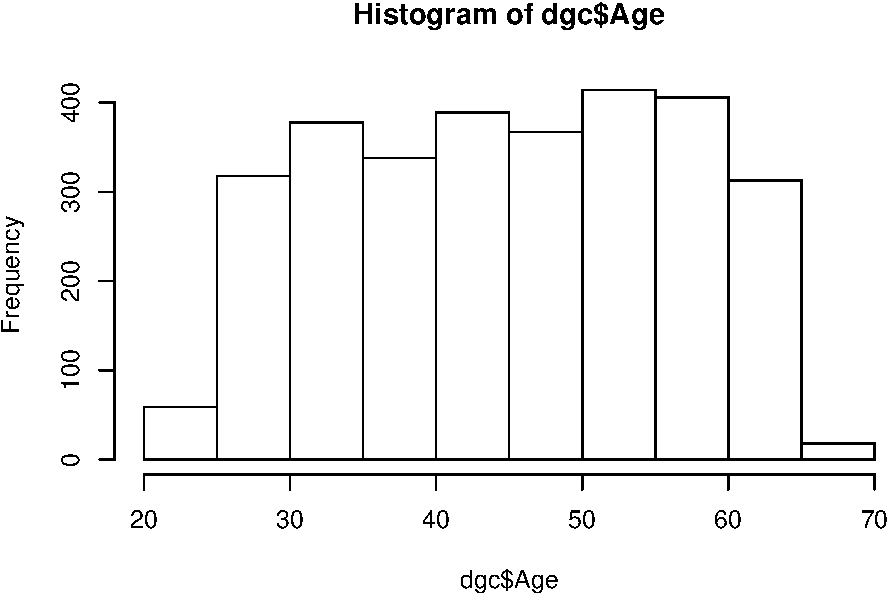
\includegraphics[width=0.3\linewidth,height=0.5\textheight]{tem_files/figure-latex/unnamed-chunk-2-1}
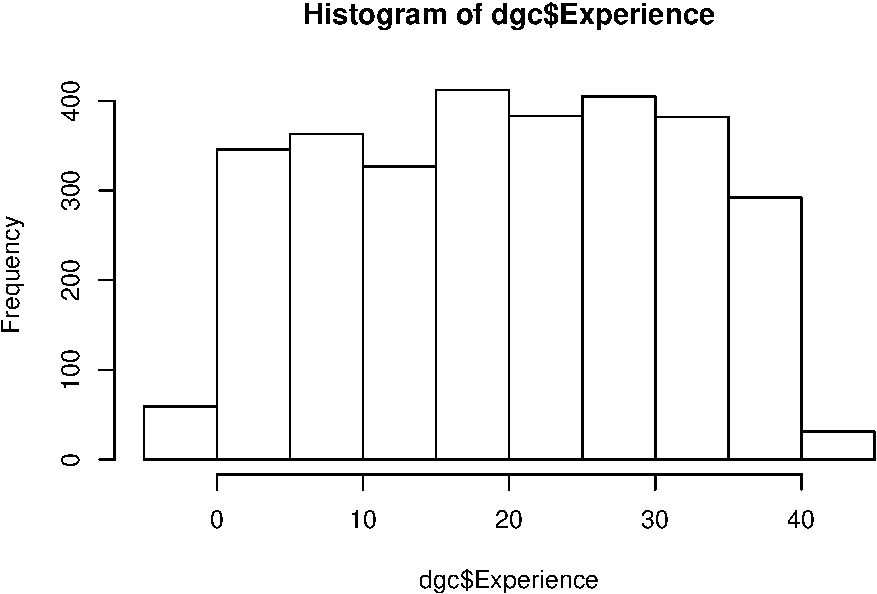
\includegraphics[width=0.3\linewidth,height=0.5\textheight]{tem_files/figure-latex/unnamed-chunk-2-2}
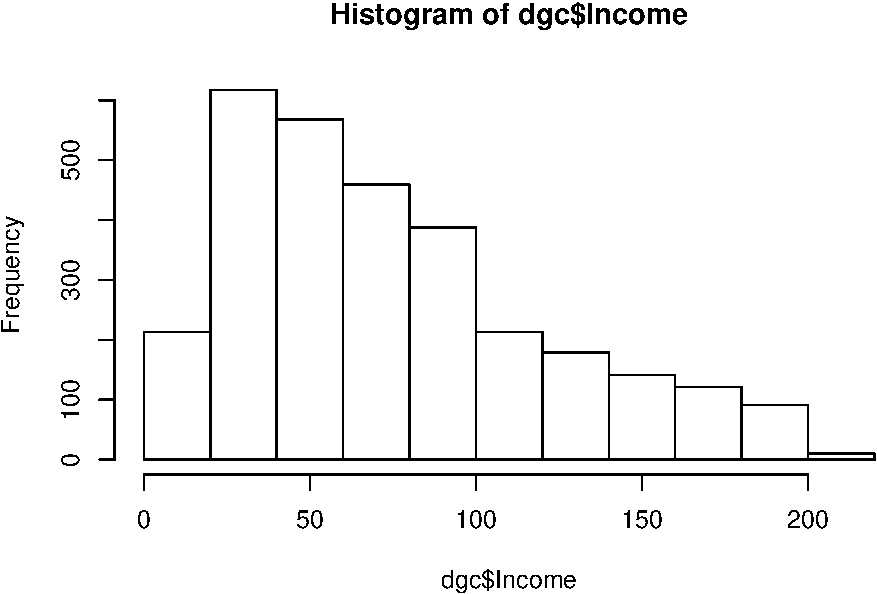
\includegraphics[width=0.3\linewidth,height=0.5\textheight]{tem_files/figure-latex/unnamed-chunk-2-3}
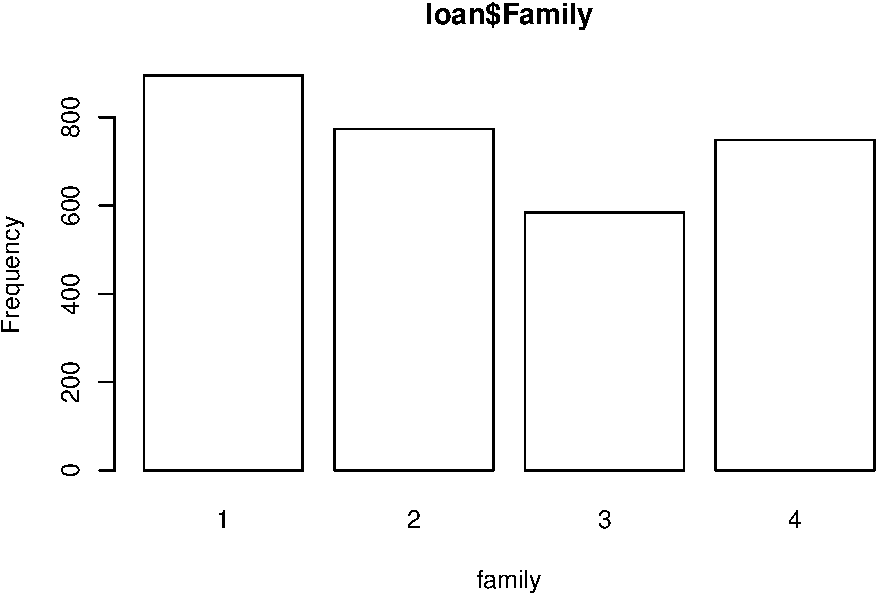
\includegraphics[width=0.3\linewidth,height=0.5\textheight]{tem_files/figure-latex/unnamed-chunk-2-4}
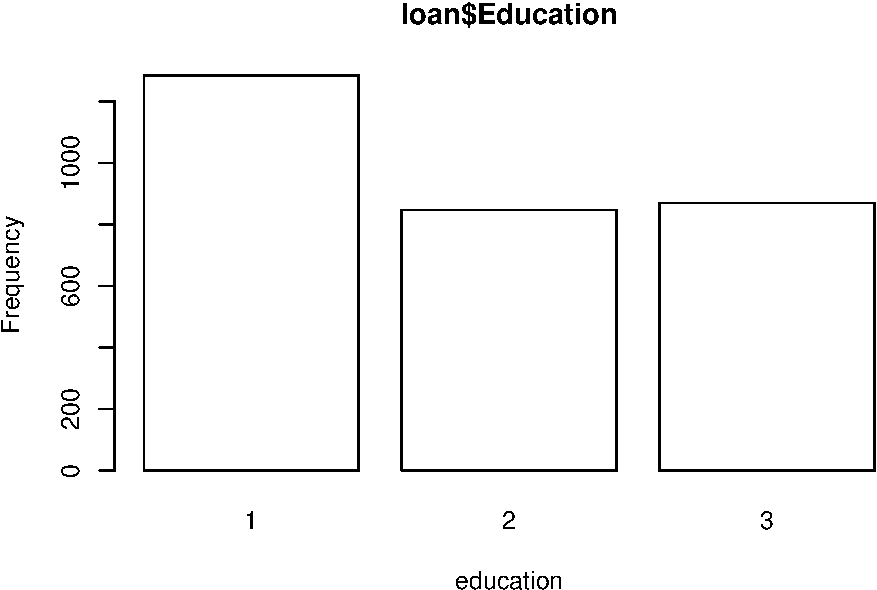
\includegraphics[width=0.3\linewidth,height=0.5\textheight]{tem_files/figure-latex/unnamed-chunk-2-5}\\

  As we can see from the histograms and bar plots, the distributions of the age and experience of the bank’s customers are smooth, varying mainly from 25-65 years and 0-40 years respectively. And the proportion of each part is similar. It shows that the bank’s customers from all backgrounds of age and working experience and there is no specific feature.\\ 
\begin{wrapfigure}{r}{0.5\textwidth} 
  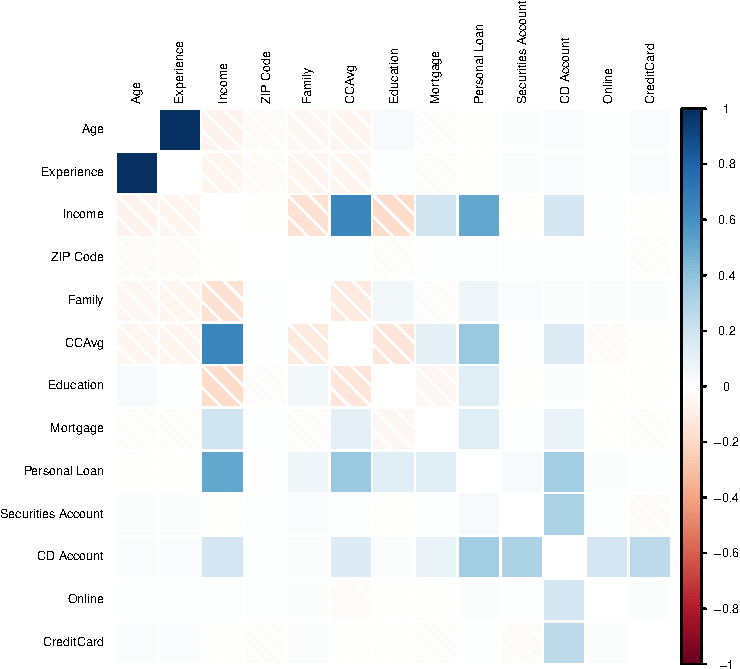
\includegraphics{tem_files/figure-latex/exa-1.pdf}
  \caption{Correalation Among Variables}
\end{wrapfigure}
  As for the income, it is obvious that the main customer group is people with annual income level from 20-100 thousand. And there is also a decreasing trend, which means with income increasing, people prefer not to open accounts in this bank. Maybe it has something to do with the bank’s positioning.\\
  In term of family size, the largest percentage of customers is people with family size of 1, followed by family size of 4. There is no special situation observed.\\
  About education, most of its customers are with bachelor’s degree, about 1/3 higher than customers with master’s degree and advanced/professional degree. The last two kinds have nearly the same amount.\\
  From the correlation plot of the five variables, it is obvious that age and experience have a strong positive correlation, which is the same with our expectation. \\
  However, it seems that family and education both have a slight negative correlation with income. Maybe people with higher income level have more advanced life insights, so some of them prefer to have fewer children. Another possible reason is that they are busy doing their career, thus have less time to take good care of families. \\
  As for education and income, it is possible that many people may think earning money is more important than obtaining a higher degree. So they prefer to earn money first and then they don’t have enough time to get a higher degree. In addition, some people may choose to learn by themselves in order to rich themselves. As a consequence, even though they don’t have a high degree, their income level is satisfied.


\subsection{(b)Analyze what variables possibly make a customer more likely to accept a personal loan?}

\begin{wrapfigure}[18]{r}{0.5\textwidth} 
  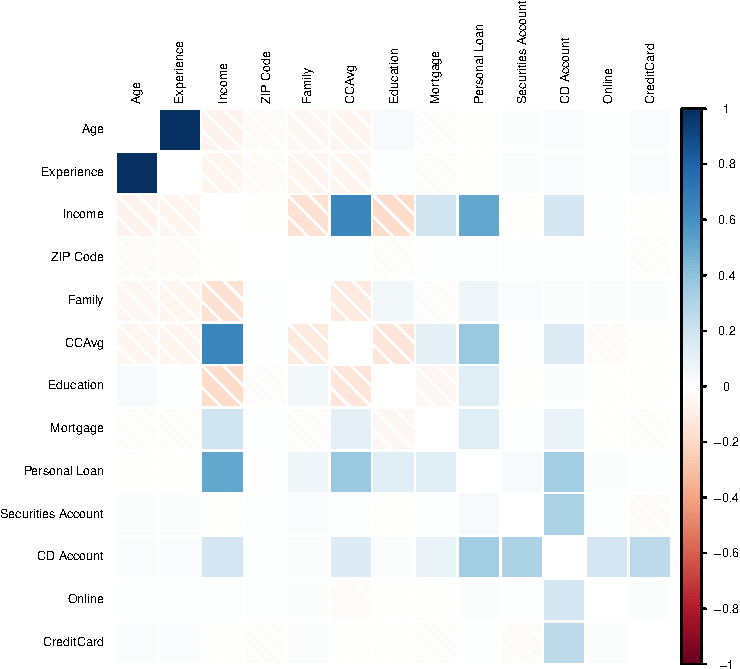
\includegraphics{tem_files/figure-latex/exa-1.pdf}
  \caption{Correalation Among Variables}
\end{wrapfigure}
In this question, we decide to analyze it in both qualitative and quantitative way. 

\textbf{(i)Qualitative Analysis:}\\
Regarding the possibility of customers to accept personal loan, the graph clearly demonstrates the correlation between personal loan and other variables. It is apparent that personal loan is positively correlated to 7 variables, which are:
\begin{itemize}
	\item Income
	\item Family
	\item CCAvg
	\item Education
	\item Mortgage
	\item Securities Account
	\item CD account
\end{itemize}

For each variable correlated to "Personal Loan", there could be some possible explanation for it. To demonstrate it more clearly, possible explanation for every variable is concluded in the table below.\\
\makeatletter\def\@captype{table}\makeatother
\begin{table}[H]
	\centering
	\caption{Summary of Personal Loan's Correlated Variables}
	\begin{tabular}{|c|c|p{10cm}|} 
	\hline
		Variable & Coefficience & Possible Explanation\\ \hline
		Income & 0.517 & (1)People who earn higher salaries will have more funding needs for investment. (2)People use personal loan for investment and consequently gain a higher income\\ \hline
		CCAvg & 0.376 & People with a higher average spending in credit card probably has a stronger sense in "pre-expenditure". This might make them: (1)run out of money so they have to use personal loan for payback. (2)get loan for future. \\ \hline
		CD Account & 0.347 & People with enough deposit are willing to accept personal loan because they at least can guarantee they have money to pay the loan partially when they CD account is due.\\ \hline
		Education & 0.137 & Education: (1) People with higher degree may have more advanced consumption concept, thus to accept personal loan and spend in advance.(2) These people may have the demand for some research equipment which is very costly.\\ \hline
		Mortgage & 0.136 & The reason seems obvious. People who need to pay for the mortgage are more likely to accept loan so that they can have enough money to maintain their daily life.\\ \hline
		Family & 0.063 & It is quite possible that people with a larger family size have stronger motivation to use personal loan. Generally, they have heavier life burden. They need to borrow money from the bank to support their family, and then work hard to pay off it.\\ \hline
		Securities Account & 0.033 & As we know, buying securities is a kind of investment. So, these people need to have enough current fund to deal with some big variance of their investments. And when they believe the market is good they want to borrow money to increasing their investment amount.\\ \hline	
	\end{tabular}
\end{table}

But we need to pay attention to the fact that the correlation can only show the linear relation between the variables. Our logistic model can reveal a more reliable relation between personal loan and other variable, not just focus on linear relation. Therefore we used \textbf{quantitative model} for further discovery.\\

\textbf{(ii)Quantitative Analysis}\\
For quantitative analysis, Logistic regression model is applied. The reason why we choose the Logistic model is that:
\begin{itemize}
	\item The dependent variable is binary variable (Y=1 or Y=0)
	\item The linear probability cannot better measure since the probability should be between 0 and 1. Logistic regression is used to describe data and to explain the relationship between one dependent binary variable and one or more nominal, ordinal, interval or ratio-level independent variables.\\
\end{itemize}
\textbf{Regression1: }\\
All variables in the model, model is shown in the screen shot from STAT.
\begin{figure}[H]
	\centering
	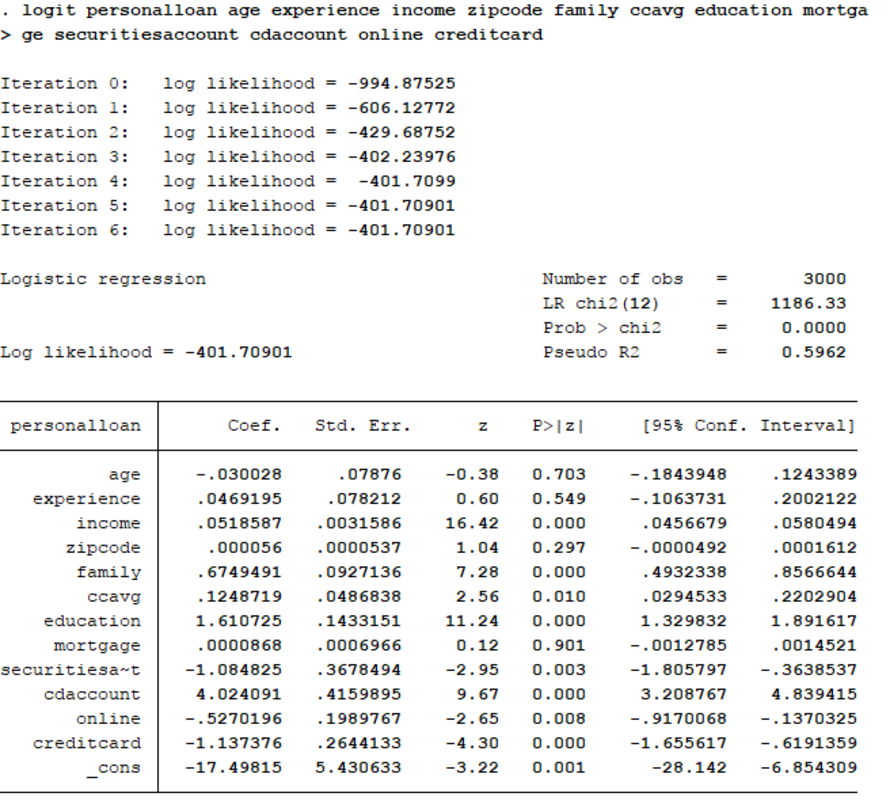
\includegraphics[width=1\linewidth,height=1\textheight]{tem_files/figure-latex/REG1.pdf}\caption{STAT Screen Shot for REG1}
\end{figure}
We figure out some of the variables are not significant because their p-value is more than 0.05. It may have imperfect multicollinearity, irrelevant variable or omitted variable. \\

\textbf{Regression2:}\\
From the correlation plot, the correlation between mortgage and income is positive relationship, and the p-value of mortgage is greater than 0.05. Thus, we decide to remove the mortgage.
\begin{figure}[H]
	\centering
	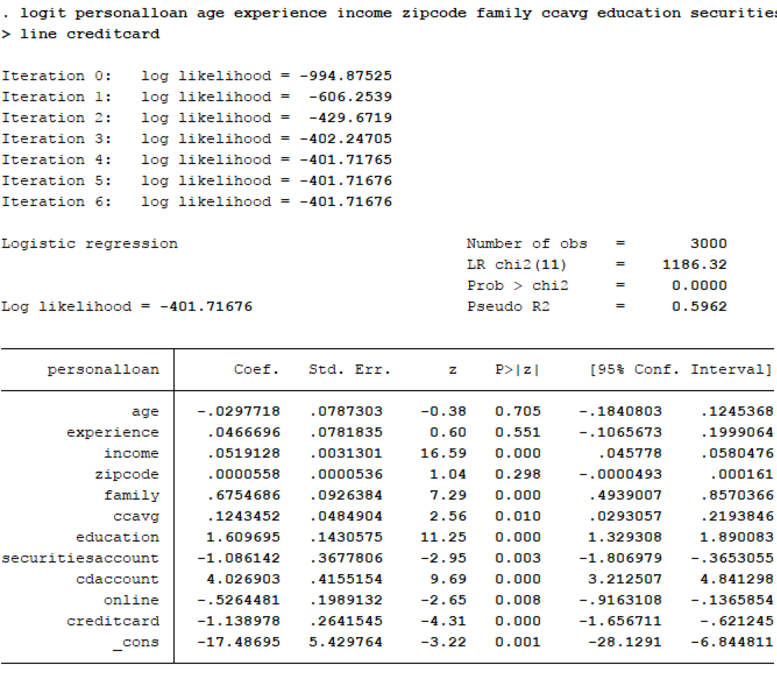
\includegraphics[width=1\linewidth,height=1\textheight]{tem_files/figure-latex/REG2.pdf}\caption{STAT Screen Shot for REG2}
\end{figure}

\textbf{Regression3}\\
Age and experience have highly positive relationship. If we put both age and experience in the model, it will affect the regression. Compared these two variables, the work experience is more meaningful to the personal loan. The age doesn’t have the clear stable relationship with personal loan since it much depends on the need of different age period. For example, when you are an adult, you may more likely to have the personal loan as the age increases. However, when you get old, you don’t want the loan in order to avoid the risk. Thus, we decide remove the age. \\
Zip code is not necessary because the coefficient is small, p-value is great than 0.05. Zip code doesn’t have the economics meaning to the personal loan. 
\begin{figure}[H]
	\centering
	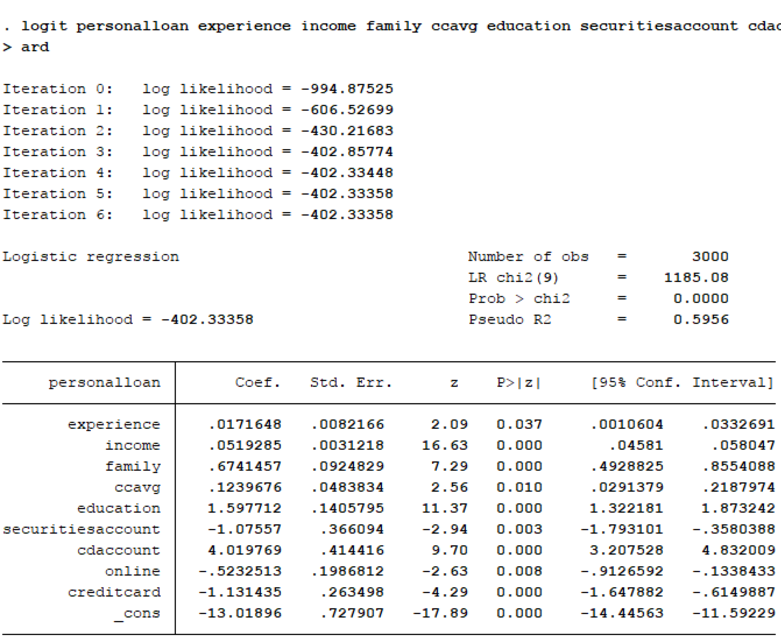
\includegraphics[width=1\linewidth,height=1\textheight]{tem_files/figure-latex/REG3.pdf}
	\caption{STAT Screen Shot for REG3}	
\end{figure}
Finally, the pseudo R square is 0.5956, which means all variables explain almost 60\% of the variance in personal loan. All the p-value are less than 0.05. They are significant. Experience, income, family, credit card average spending, education and CD account have positive relationship with the personal loan. Securities account, online banking and credit card have negative relationship with the personal loan. CD account is much more significant than the other variables because if you have CD account, you have more ability to pay back the personal loan in the future. What’s more, the bank may promote the advertisement of personal loan to the customers who have the CD account.

\begin{figure}[H]
	\centering
	\begin{minipage}{0.48\textwidth}
	\centering
		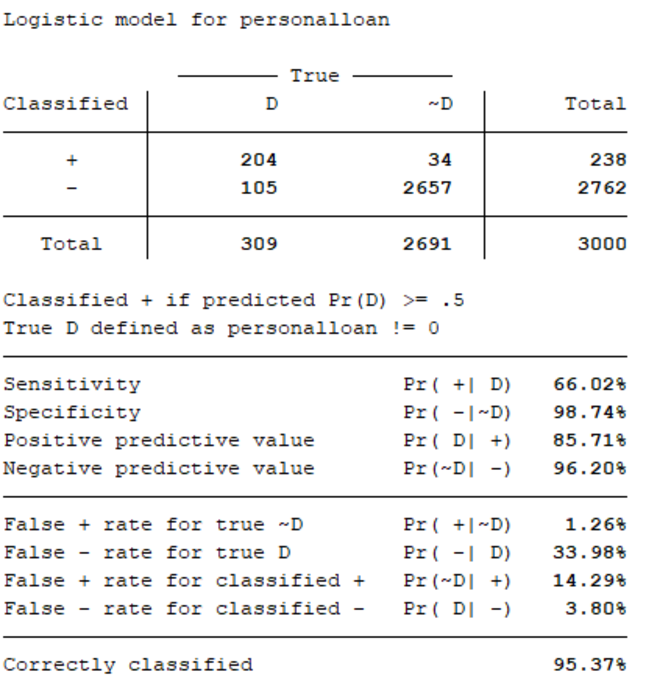
\includegraphics{tem_files/figure-latex/REG3-1.pdf}
		\caption{Model}
	\end{minipage}
	\begin{minipage}{0.48\textwidth}
	\centering
		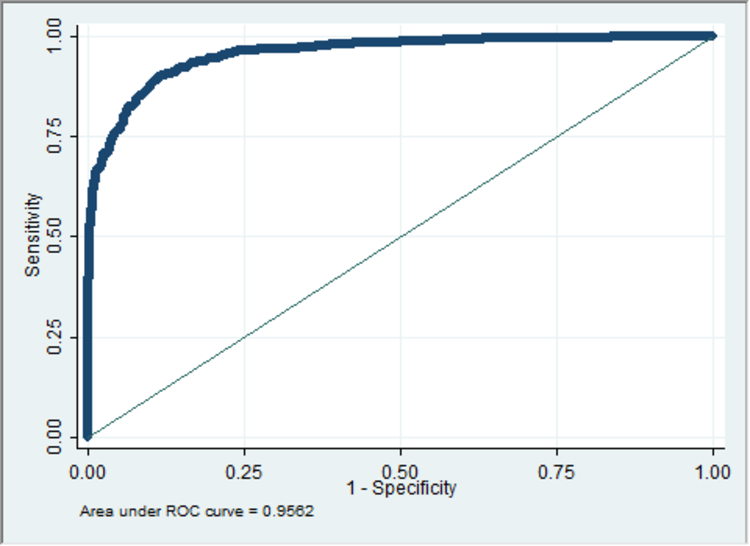
\includegraphics{tem_files/figure-latex/REG3-2.pdf}
		\caption{ROC Curve}
	\end{minipage}
\end{figure}

A receiver operating characteristic curve, (ROC curve), is a graphical plot that illustrates the diagnostic ability of a binary classifier system as its discrimination threshold is varied.

The best possible prediction method would yield a point in the upper left corner or coordinate (0,1) of the ROC space, representing 100\% sensitivity and 100\% specificity. The (0,1) point is also called a perfect classification. A random guess would give a point along a diagonal line from the left bottom to the top right corners.

In this case, our correctly classified is 95.37\%. our ROC curve closes to the (0,1) point, and the area under ROC curve is 0.9552. 

In conclusion, from our model, \textbf{experience, income, family, credit card average spending, education, securities account, cd account, online banking, credit card} possibly makes a customer more likely to accept a personal loan.

\subsection{(c)There are several products the bank offers like CD and security accounts, online services, credit cards, etc. Can we identify any association among these for finding cross-selling opportunities?}
To identify cross-selling opportunities, here we try to use \textbf{shopping basket analysis} to discover cross-selling rules for different products. During the analysis, we regard there are 6 products :\textbf{Mortgage, Personal Loan, Securities Account, CD Account, Online} and \textbf{Credit Card}. Among the variables, mortgage is the only numeric variable. Therefore, we change it as a nominal variable, which represents whether have mortgage. \\

Before running advanced model, we could use bar plot to check the most frequent bought item

\begin{figure}[H]
	\centering
	\begin{minipage}{0.28\textwidth}
	\centering
		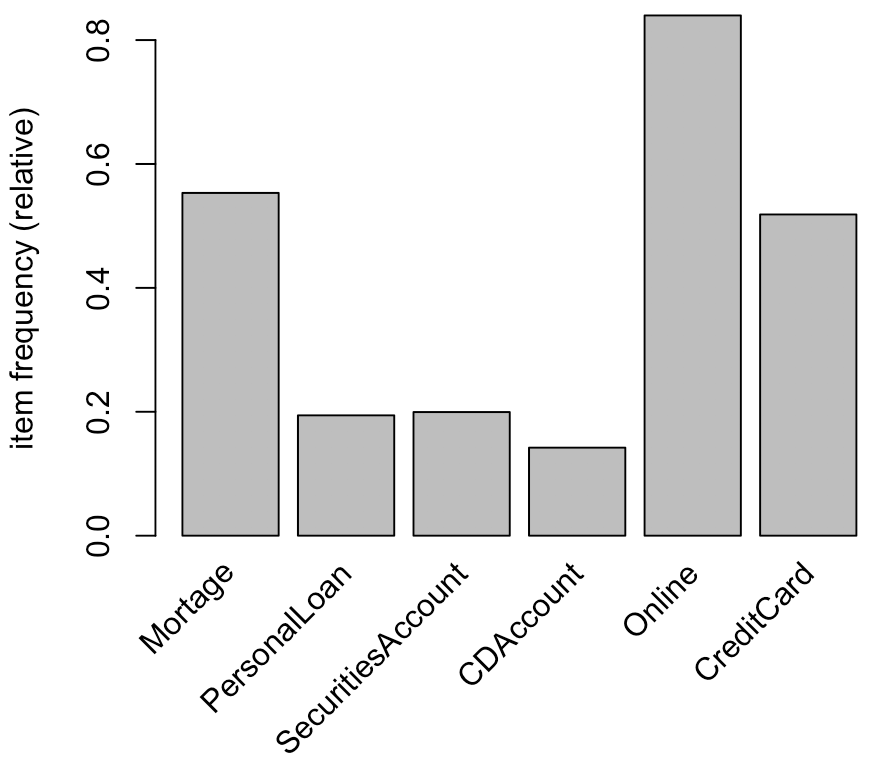
\includegraphics{tem_files/figure-latex/shopbasket-4.png}
		\caption{Item Frequency Plot}
	\end{minipage}
	\hspace{1cm}
	\begin{minipage}{0.60\textwidth}
As shown in the graph, online services has the highest relative frequency, indicating that it is the best selling product among other products. \textbf{This means that online services could probably be sold together with other products.}\\ 
On the other hand, CDAccount has the lowest relative Frequency, indicating that might be the least popular product compared to other products offered by bank.
	\end{minipage}
\end{figure}


We set we set the \textbf{Confidence level at 0.1, Support at 0.1}. After running Shopping Basket Analysis Model, we found 20 rules in total. Sorted by \textbf{lift}, the top 6 is demonstrated as below:
\makeatletter\def\@captype{table}\makeatother
\begin{table}[H]
	\centering
	\caption{Summary of Association Rules Among Different Products}
	\begin{tabular}{|c|c|c|c|c|c|} 
	\hline
		No. & LHS & RHS & Support & Confidence & Lift\\ \hline
		1 & Online, CreditCard & CDAccount & 0.1005291 & 0.2504708 & 1.762622\\ \hline
		2 & CDAccount, Online & CreditCard & 0.1005291 & 0.7471910 & 1.441011\\ \hline
		3 & CDAccount & CreditCard & 0.1058201 & 0.7446809 & 1.436170\\ \hline
		4 & CreditCard & CDAccount & 0.1058201 & 0.2040816 & 1.436170\\ \hline
		5 & CDAccount, CreditCard & Online & 0.1005291 & 0.9500000 & 1.131278\\ \hline
		6 & Online & CDAccount & 0.1345427 & 0.1602160 & 1.127478\\ \hline
	\end{tabular}
\end{table}

In shopping basket model, lift indicates the possibly that the presence of items in LHS will trigger the occurance of items in RHS. For lift greater than 1, it suggests that the precense of the items on the LHS increase the probability that the items on the right hand side will occur on this transaction. \\
For instance, the first rule \{Online,CreditCard\}=>\{CDAccount\} has a lift near 1.76, meaning that client who use Online Services and Credit Card will tend to apply for a Cash Deposit Account. 
To demonstrate the association rules more clearly, we can use network graph and parallel coordinates plot.

\begin{figure}[H]
	\centering
	\begin{minipage}{0.58\textwidth}
	\centering
		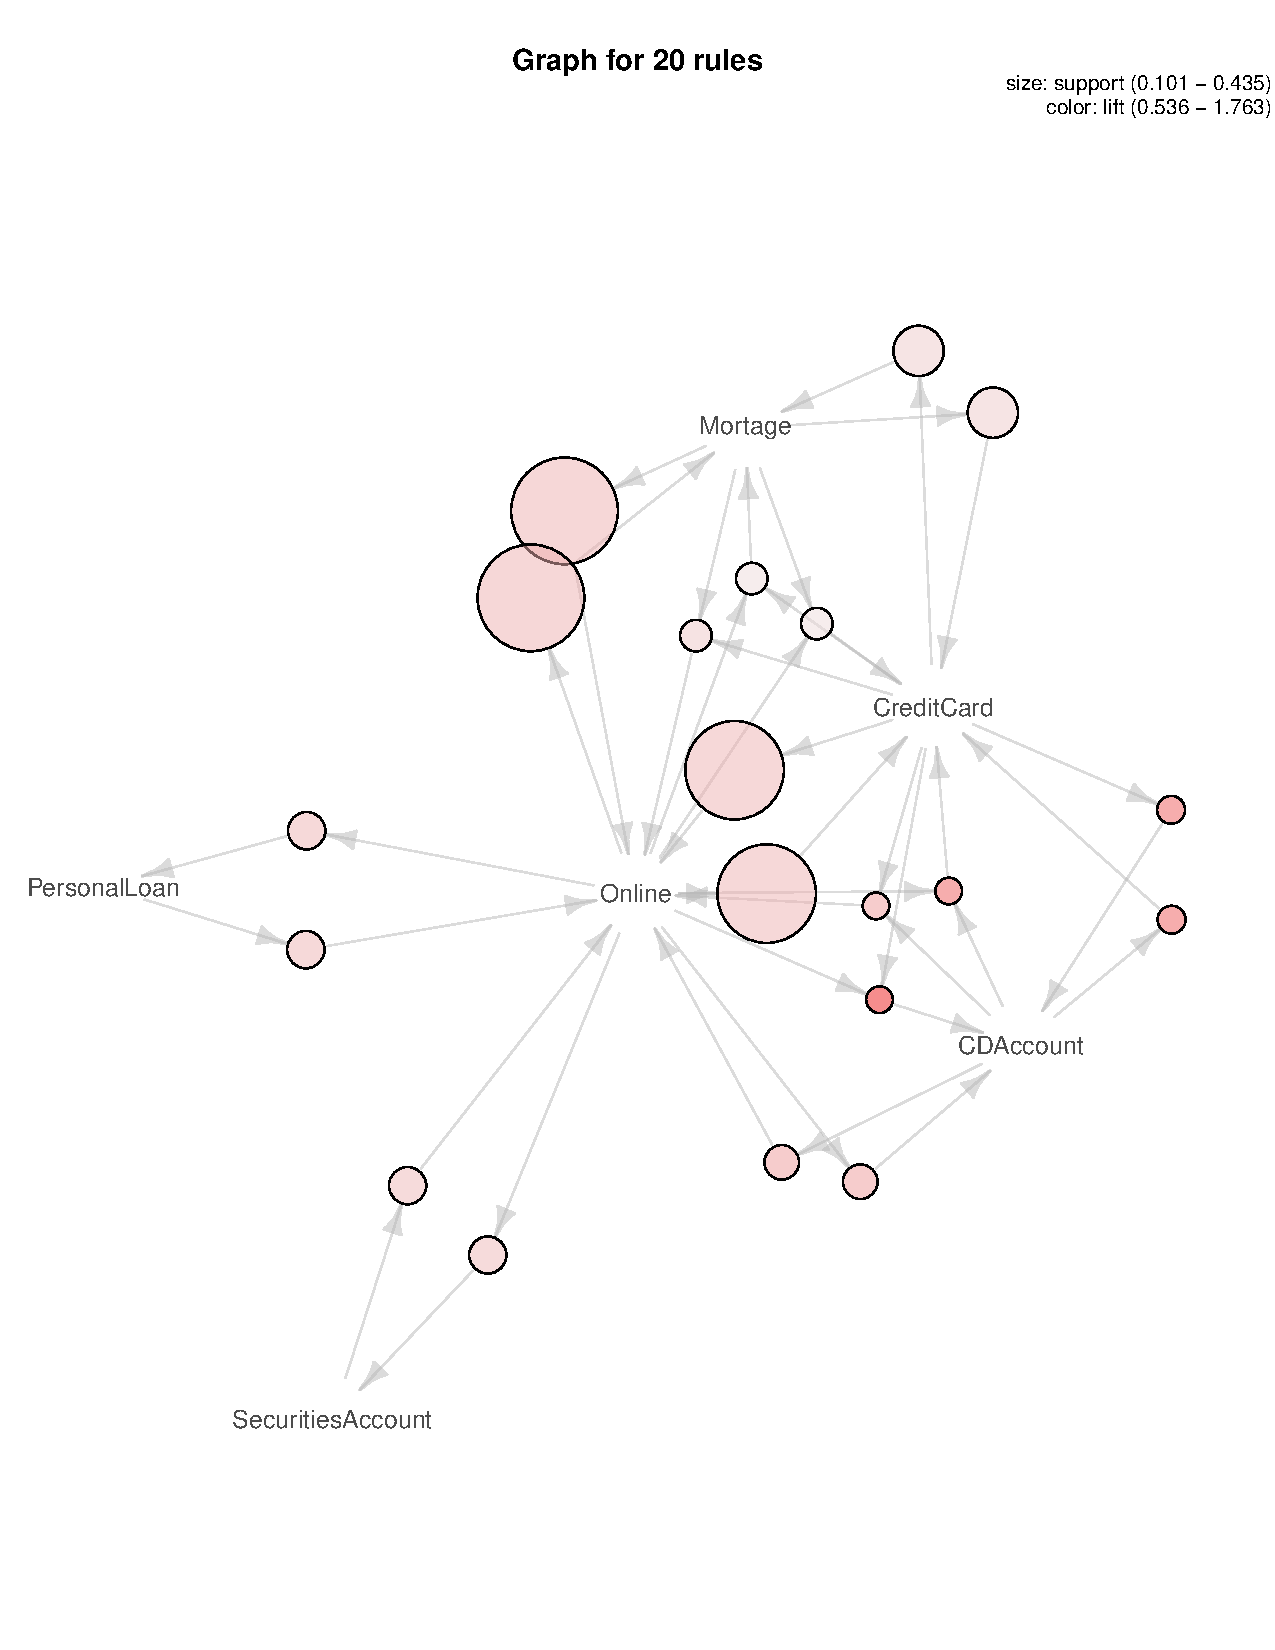
\includegraphics{tem_files/figure-latex/shopbasket-1.pdf}
		\caption{Network Graph}
	\end{minipage}
	\hspace{1cm}
	\begin{minipage}{0.28\textwidth}
As shown in the graph, the size of the circle represents represents the rules' support(the larger, the greater), while the color of the circle represents rules' lift (the deeper, the greater)\\
From the network graph, we can see that \textbf{Online Services, Mortgage, CreditCard} and \textbf{CDAccount} are most frequently related to other products. \textbf{This might indicate that these products could be bonded to a wide range of products for cross-selling.} 
	\end{minipage}
\end{figure}

\begin{figure}[H]
	\centering
	\begin{minipage}{0.58\textwidth}
	\centering
		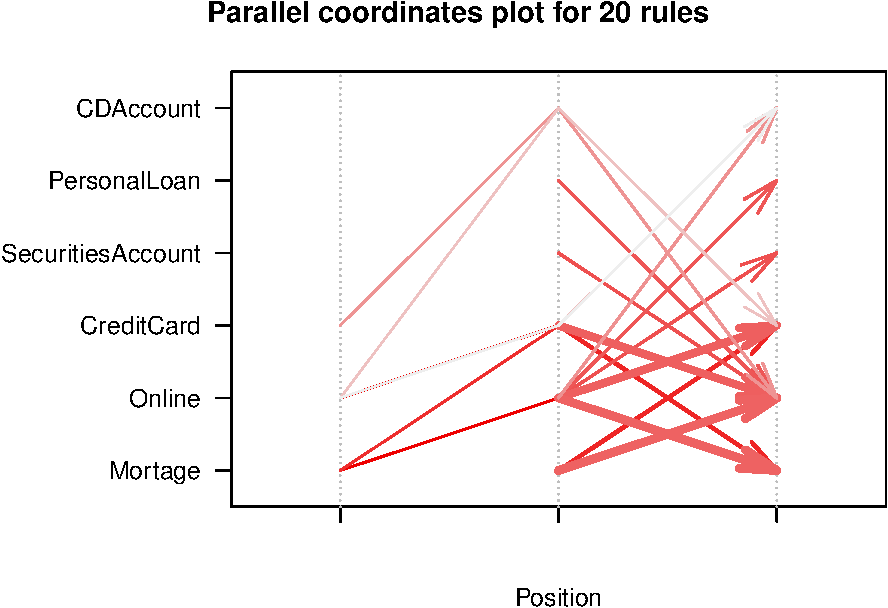
\includegraphics{tem_files/figure-latex/shopbasket-2.pdf}
		\caption{Parallel Coordinate Plot}
	\end{minipage}
	\hspace{1cm}
	\begin{minipage}{0.28\textwidth}
As shown in the graph, different directed lines represent different rules(from LHS to RHS). Thicker line represents a higher support, while a deeper color represents a higher lift.  \\
From the network graph, we can see that \textbf{Online Services, CreditCard} and \textbf{Mortgage} are most frequently directed to by other products. And some of the rules lines are and in deep color. \textbf{This might indicate that these products could be sold as add-in or promotion when selling other products to customers.}
	\end{minipage}
\end{figure}


\end{document}
